\paragraph{Coding relative to the initialization.} \Cref{tab:init} trains the same 784--256--10 network from three initialization scales and from a deterministic DCT initialization, and codes the update either relative to the (free) initialization or relative to zero, with the unlabeled-data codec of \cref{sec:exp-t2}. \Cref{tab:t3} makes the same comparison for the dithered training-data-only code of a 32-unit network: coding relative to zero costs 84{,}269 bits against 83{,}976, a difference of 0.3\%. Two effects explain why the initialization matters so little here. First, Adam moves the first-layer weights far from their initial values, so the update is not small compared with the initialization. Second, in the dithered code the steps in the high-frequency DCT bands are coarse, because natural images have little energy there, so describing the random initial weights in those bands costs almost nothing. The deterministic DCT initialization, which costs nothing either, led to a more compressible network: 67k bits against 84k.

\begin{table}[t]
\centering\small
\begin{tabular}{l r l r r r r r}
\toprule
initialization & scale & code relative to & test err.\ $f$ & bound on $g$ & bits & bound on $f$ & bits \\
\midrule
seeded random & 0.3 & initialization & 0.0199 & 0.384 & 34421 & 0.407 & 34421 \\
seeded random & 1 & initialization & 0.0197 & 0.367 & 32264 & 0.391 & 32264 \\
seeded random & 1 & zero & 0.0197 & 0.377 & 34095 & 0.399 & 34095 \\
\bottomrule
\end{tabular}
\caption{MNIST, 784-256-10: description length and bounds when the update is coded relative to the (free) initialization or relative to zero, for three initialization scales and a deterministic initialization. Best of 8 compression configurations each.}\label{tab:init}
\end{table}


\paragraph{The init-kernel codec in the lazy and rich regimes.} \Cref{tab:kernel} compares, on the same Boolean networks ($n=30$, one hidden layer of 512 units), the init-kernel codec of \cref{prop:kernel} with function-space distillation. The lazy regime uses initialization scale 2 and plain SGD; the parameters then move by about 10\% of their initial norm, and $f$ agrees with its linearization at $\theta_0$ on 97--99.9\% of inputs. The rich regime uses scale 0.1 and Adam; the parameters move by 3--5 times their initial norm and the linearization is poor. The init-kernel codec describes $\theta_0+P_r\Delta$, where $P_r$ projects onto the top-$r$ eigenvectors of the uniform-input empirical kernel at $\theta_0$. That kernel is estimated from 4000 uniform inputs, so it is free given $\theta_0$. The candidate ranks include the dimensions of the low-degree Walsh spaces: $1+n=31$, $1+n+\binom n2=466$ and $4526$.

The results match the picture of \cref{sec:init-theory}.
\begin{itemize}
\item In the lazy regime the best rank is the dimension of the low-degree Walsh space that the target lives in. For the majority targets it is exactly $r=31$, the dimension of the functions of degree at most 1, and the bounds are 0.05--0.25. For the degree-2 target \texttt{parity2} it is exactly $r=466$, the dimension of degree at most 2. Describing 466 coefficients costs about 1500 bits, so the bound is still 0.59 at $m=4000$; the distilled junta needs 20 bits and gets 0.006. The estimated bound as a function of $r$ has a sharp minimum at these dimensions (\cref{fig:kernel}). This is the $n^k$ sample complexity of kernel methods appearing as description length.
\item In the rich regime the update is far from the initial kernel's top eigenspace and the codec fails.
\item Function-space distillation does better in both regimes. It describes the function, not the update, so how far training moved from the initialization does not matter to it.
\end{itemize}

\begin{table}[t]
\centering\small
\begin{adjustbox}{max width=\linewidth}\begin{tabular}{l l r r r r r r r r}
\toprule
task & regime & $m$ & test err.\ $f$ & move & lin.\ dis. & $r$ & bits & init-kernel bound & distillation bound \\
\midrule
\texttt{fullmaj} & lazy & 1000 & 0.0387 & 0.11 & 0.015 & 31 & 205 & 0.253 & 0.080 \\
\texttt{fullmaj} & rich & 1000 & 0.0000 & 4.57 & 0.346 & 16 & 124 & 0.821 & 0.036 \\
\texttt{fullmaj} & lazy & 4000 & 0.0039 & 0.17 & 0.032 & 31 & 241 & 0.143 & 0.013 \\
\texttt{fullmaj} & rich & 4000 & 0.0000 & 4.71 & 0.277 & 31 & 196 & 0.502 & 0.009 \\
\texttt{maj5} & lazy & 1000 & 0.0010 & 0.09 & 0.002 & 31 & 208 & 0.158 & 0.033 \\
\texttt{maj5} & rich & 1000 & 0.0000 & 3.32 & 0.080 & 31 & 170 & 0.288 & 0.032 \\
\texttt{maj5} & lazy & 4000 & 0.0003 & 0.09 & 0.001 & 31 & 214 & 0.052 & 0.009 \\
\texttt{maj5} & rich & 4000 & 0.0000 & 3.98 & 0.197 & 31 & 213 & 0.297 & 0.008 \\
\texttt{parity2} & lazy & 1000 & 0.0181 & 0.17 & 0.168 & 466 & 1519 & 0.940 & 0.039 \\
\texttt{parity2} & rich & 1000 & 0.0000 & 3.58 & 0.434 & 2048 & 8230 & 1.000 & 0.020 \\
\texttt{parity2} & lazy & 4000 & 0.0003 & 0.18 & 0.133 & 466 & 1524 & 0.591 & 0.006 \\
\texttt{parity2} & rich & 4000 & 0.0000 & 3.53 & 0.410 & 2048 & 6094 & 0.772 & 0.005 \\
\bottomrule
\end{tabular}\end{adjustbox}
\caption{Boolean tasks ($n=30$, one hidden layer of 512): the init-kernel codec of \cref{prop:kernel} ($\theta_0$ plus the top-$r$ eigenvectors of the uniform-input empirical NTK at $\theta_0$, both free) against function-space distillation, on the same networks. `Move': $\|\theta-\theta_0\|/\|\theta_0\|$; `lin.\ dis.': disagreement between $f$ and its linearization at $\theta_0$. One seed per row.}\label{tab:kernel}
\end{table}


\begin{figure}[t]
\centering
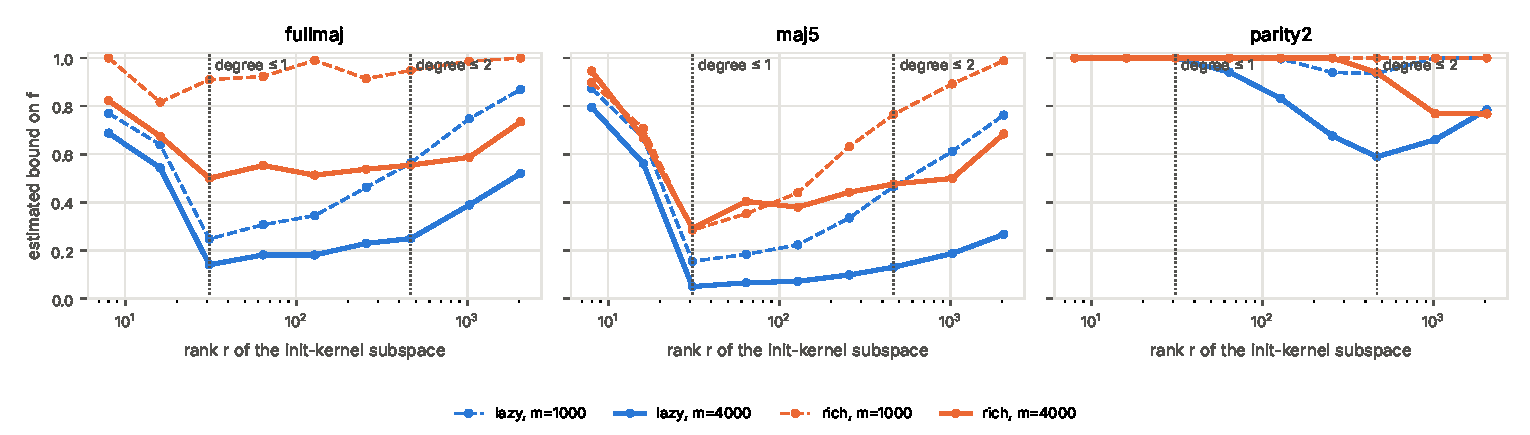
\includegraphics[width=\linewidth]{../figures/init_kernel.pdf}
\caption{Init-kernel codec: estimated bound on $f$ (Occam term plus disagreement on a selection pool) as a function of the rank $r$ of the subspace spanned by the top eigenvectors of the initial kernel, for networks trained in the lazy (blue) and rich (orange) regimes. Dotted lines: dimensions of the Walsh spaces of degree at most 1 ($1+n$) and at most 2 ($1+n+\binom n2$).}\label{fig:kernel}
\end{figure}
